%% 11/23/2015
%%%%%%%%%%%%%%%%%%%%%%%%%%%%%%%%%%%%%%%%%%%%%%%%%%%%%%%%%%%%%%%%%%%%%%%%%%%%
% AGUJournalTemplate.tex: this template file is for articles formatted with LaTeX
%
% This file includes commands and instructions
% given in the order necessary to produce a final output that will
% satisfy AGU requirements. 
%
% You may copy this file and give it your
% article name, and enter your text.
%
%%%%%%%%%%%%%%%%%%%%%%%%%%%%%%%%%%%%%%%%%%%%%%%%%%%%%%%%%%%%%%%%%%%%%%%%%%%%
% PLEASE DO NOT USE YOUR OWN MACROS
% DO NOT USE \newcommand, \renewcommand, or \def, etc.
%
% FOR FIGURES, DO NOT USE \psfrag or \subfigure.
% DO NOT USE \psfrag or \subfigure commands.
%%%%%%%%%%%%%%%%%%%%%%%%%%%%%%%%%%%%%%%%%%%%%%%%%%%%%%%%%%%%%%%%%%%%%%%%%%%%
%
% Step 1: Set the \documentclass
%
% There are two options for article format:
%
% 1) PLEASE USE THE DRAFT OPTION TO SUBMIT YOUR PAPERS.
% The draft option produces double spaced output.
% 
% 2) numberline will give you line numbers.

%% To submit your paper:
\documentclass[draft,linenumbers]{agujournal}
% \draftfalse
\drafttrue

%% For final version.
% \documentclass{agujournal}

% Now, type in the journal name: \journalname{<Journal Name>}

% ie, \journalname{Journal of Geophysical Research}
%% Choose from this list of Journals:
%
% JGR-Atmospheres
% JGR-Biogeosciences
% JGR-Earth Surface
% JGR-Oceans
% JGR-Planets
% JGR-Solid Earth
% JGR-Space Physics
% Global Biochemical Cycles
% Geophysical Research Letters
% Paleoceanography
% Radio Science
% Reviews of Geophysics
% Tectonics
% Space Weather
% Water Resource Research
% Geochemistry, Geophysics, Geosystems
% Journal of Advances in Modeling Earth Systems (JAMES)
% Earth's Future
% Earth and Space Science
%
%

\journalname{Water Resource Research}


\begin{document}

%% ------------------------------------------------------------------------ %%
%  Title
% 
% (A title should be specific, informative, and brief. Use
% abbreviations only if they are defined in the abstract. Titles that
% start with general keywords then specific terms are optimized in
% searches)
%
%% ------------------------------------------------------------------------ %%

% Example: \title{This is a test title}

\title{When does vapor pressure deficit drive or reduce evapotranspiration?}

%% ------------------------------------------------------------------------ %%
%
%  AUTHORS AND AFFILIATIONS
%
%% ------------------------------------------------------------------------ %%

% Authors are individuals who have significantly contributed to the
% research and preparation of the article. Group authors are allowed, if
% each author in the group is separately identified in an appendix.)

% List authors by first name or initial followed by last name and
% separated by commas. Use \affil{} to number affiliations, and
% \thanks{} for author notes.  
% Additional author notes should be indicated with \thanks{} (for
% example, for current addresses). 

% Example: \authors{A. B. Author\affil{1}\thanks{Current address, Antartica}, B. C. Author\affil{2,3}, and D. E.
% Author\affil{3,4}\thanks{Also funded by Monsanto.}}

\authors{A. Massmann\affil{1}, P. Gentine\affil{1}, C. Lin\affil{2}}


% \affiliation{1}{First Affiliation}
% \affiliation{2}{Second Affiliation}
% \affiliation{3}{Third Affiliation}
% \affiliation{4}{Fourth Affiliation}

\affiliation{1}{Department of Earth and Environmental Engineering, Columbia University, New York, NY 10027}
\affiliation{2}{Department of Hydraulic Engineering, Tsinghua University, Beijing, CN}

  % (repeat as many times as is necessary)

%% Corresponding Author:
% Corresponding author mailing address and e-mail address:

% (include name and email addresses of the corresponding author.  More
% than one corresponding author is allowed in this LaTeX file and for
% publication; but only one corresponding author is allowed in our
% editorial system.)  

% Example: \correspondingauthor{First and Last Name}{email@address.edu}

\correspondingauthor{Adam Massmann}{akm2203@columbia.edu}

%% Keypoints, final entry on title page.

% Example: 
% \begin{keypoints}
% \item	List up to three key points (at least one is required)
% \item	Key Points summarize the main points and conclusions of the article
% \item	Each must be 100 characters or less with no special characters or punctuation 
% \end{keypoints}

%  List up to three key points (at least one is required)
%  Key Points summarize the main points and conclusions of the article
%  Each must be 100 characters or less with no special characters or punctuation 

\begin{keypoints}
\item = enter point 1 here = 
\item = enter point 2 here = 
\item = enter point 3 here = 
\end{keypoints}

%% ------------------------------------------------------------------------ %%
%
%  ABSTRACT
%
% A good abstract will begin with a short description of the problem
% being addressed, briefly describe the new data or analyses, then
% briefly states the main conclusion(s) and how they are supported and
% uncertainties. 
%% ------------------------------------------------------------------------ %%

%% \begin{abstract} starts the second page 

\begin{abstract}
= enter abstract here =
\end{abstract}


%% ------------------------------------------------------------------------ %%
%
%  TEXT
%
%% ------------------------------------------------------------------------ %%

%%% Suggested section heads:
% \section{Introduction}
% 
% The main text should start with an introduction. Except for short
% manuscripts (such as comments and replies), the text should be divided
% into sections, each with its own heading. 

% Headings should be sentence fragments and do not begin with a
% lowercase letter or number. Examples of good headings are:

% \section{Materials and Methods}
% Here is text on Materials and Methods.
%
% \subsection{A descriptive heading about methods}
% More about Methods.
% 
% \section{Data} (Or section title might be a descriptive heading about data)
% 
% \section{Results} (Or section title might be a descriptive heading about the
% results)
% 
% \section{Conclusions}


\section{Introduction}\explain{This section needs to be fleshed out, and I definately need to add more citations}

Changes to vapor pressure deficit (VPD) alter the atmospheric demand for water from the land surface. However, plant stomata have evolved to optimally regulate the exchange of water and carbon between vegetation and the atmosphere \citep{Franks_2017}. Therfore, an increase (decrease) in VPD may not correspond to an increase (decrease) in evapotranspiration (ET) because stomatal closure (opening) can cancel the effects of shifts to atmospheric demand.

Quantifying the plant response to a perturbation to atmospheric VPD increases our understanidng of feedbacks between the land surface and the atmosphere. If plant reponse reduces ET in response to an increase in VPD, the land surface will contribute a positive feedback in reponse to atmospheric drying. Conversely, if plant response increases ET in response to increase in VPD, then the land surface will contribute a negative feedback to atmospheric drying. The sign of these feedbacks drives the evolution of the atmosphere and landsurface at many timescales, from diurnal to interdecadal. 

Here we use a Penman-Monteith framework to quantify plant reponse to perturbations to atmospheric demand for water. Section 2 derives the framework, Section 3 describes the data used, Section 4 presents results, and Section 5 discusses conclusions. The goal of this paper is to use reasonable approximations as a tool to increase intuition for plant response to atmospheric drying. This intuition will aid interpretation of observations and full complexity climate models.

\section{Methods}

The Penman-Monteith equation (hereafter PM) estimates ET as a function of atmospheric and land-surface variaibles:

\begin{linenomath*}
  \begin{equation}
      ET = \frac{\Delta R + g_a \rho_a c_p D_{s}}{\Delta + \gamma(1 + \frac{g_a}{g_s})},
  \end{equation}
\end{linenomath*}

 where variable definitions are given in Table 1. \cite{MEDLYN_2011} developed a model for $g_s$ by combining optimal photosynthesis theory with empiracle approaches. The result for leaf-scale stomatal resistance was:

\begin{linenomath*}
  \begin{equation}
  g_{l-s} = g_0 + 1.6 \left(1 + \frac{g_1}{\sqrt{D_{s}}}\right) \frac{A}{c_s}
  \end{equation}
\end{linenomath*}

This can be adapted to an ecosystem-scale stomatal resistance by multiplying by leaf area index (LAI) and converting units to m s$^{-1}$:
\begin{linenomath*}
  \begin{equation}
  g_s = \text{LAI } \frac{R* T}{P} \left( g_0 + 1.6 \left(1 + \frac{g_1}{\sqrt{D_{s}}}\right) \frac{A}{c_s}\right)
  \end{equation}
\end{linenomath*}

While Equation 3 can be used in PM, it will make analytical work with the function intractable because $A$ is a relatively strong function of ET. To remove dependence of ET on $A$ we can use the semi-impiracle results of \cite{Zhou_2015}. \cite{Zhou_2015} showed that:

\begin{linenomath*}
  \begin{equation}
uWUE = \frac{GPP \cdot \sqrt{D}}{ET}
  \end{equation}
\end{linenomath*}
is relatively constant across time and space (within plant functional type). If, following \cite{Lin_2015}, we approximate $g_0$ as $0$, we can use uWUE to remove $A$ from $g_s$ in a way that makes PM analytically tractable:

\begin{linenomath*}
  \begin{equation}
  g_s = \text{LAI } \frac{R* T}{P} 1.6 \left(1 + \frac{g_1}{\sqrt{D_{s}}}\right) \frac{uWUE \; ET}{c_s \; \sqrt{D}}
  \end{equation}
\end{linenomath*}

Plugging Equation 5 into Equation 1 and rearranging gives:

\begin{linenomath*}
  \begin{equation}
  ET = \frac{\Delta R + \frac{g_a\; P}{T} \left( \frac{ c_p D_{s}}{R_{air}} - \frac{\gamma c_s \sqrt{D} }{\text{LAI } R* \; 1.6 \text{ uWUE } (1 + \frac{g_1}{\sqrt{D}})} \right) }{ \Delta + \gamma}
  \end{equation}
\end{linenomath*}

We can then take the derivative with respect to $D$ to determine ecosystem reponse to atmospheric demand perturbations:

\begin{linenomath*}
  \begin{equation}
    \frac{\partial \;  ET}{\partial \; D} = \frac{g_a \; P}{T(\Delta + \gamma)}   \left(\frac{ c_p}{R_{air}} - \frac{\gamma c_s }{\text{LAI }1.6 \; R\; \text{ uWUE }} \left( \frac{2 g_1 + \sqrt{D}}{2 (g_1 + \sqrt{D})^2}\right) \right)
    \label{d_et}
  \end{equation}
\end{linenomath*}
Note that given yearly uWUE from \cite{Zhou_2015}, $g_1$ from \cite{Lin_2015} \citep[as presented in ][]{Franks_2017}, and observations of R, T, P, D$_s$, and wind speed (WS), the only unknown is LAI. With flux tower observations of ET, LAI will then be uniquely determined for each observation through Equation 6:

\begin{linenomath*}
  \begin{equation}
    LAI  = - \frac{g_a \gamma c_s \sqrt{D_s} P }{ \left(\text{ ET } ( \Delta + \gamma) - \Delta R - g_a \rho_a c_p D_{s}\right) 1.6 \; R\; T\; \text{ uWUE } (1 + \frac{g_1}{\sqrt{D_s}})}
    \label{lai}
  \end{equation}
\end{linenomath*}

This ``pseudo-LAI'' is some part ``true'' LAI (a measure of leaf area), and some part model and observational error, including error involving our assumption of constant uWUE. By calculating a unique LAI for each observation we will progate any model and observational uncertainty forward into our expression for $\frac{\partial \; ET}{\partial D}$. 


\begin{table}
\caption{Definition of symbols and variables}
\centering
\begin{tabular}{l c c}
\hline
 Variable & Description & Units  \\
\hline
$e_s$  & saturation vapor pressure & Pa  \\ 
$T$  & temperature  & K \\
$\Delta$  & $\frac{\partial e_s}{\partial T}$ & Pa K$^{-1}$ \\
$R$  & net radiation at land surface minus ground heat flux & W m$^{-2}$   \\
  $g_a$  & atmospheric conductance & m s$^{-1}$  \\
  $\rho_a$  & air density & kg m$^{-3}$  \\
  $c_p$  & specific heat capacity of air at constant pressure & J K$^{-1}$ kg$^{-1}$ \\
  $D$  & VPD & Pa  \\
  $\gamma$  & psychrometric constant & Pa K$^{-1}$   \\
  $g_s$  & stomatal conductance & m s$^{-1}$  \\
  $g_{l-s}$  & leaf-scale stomatal conductance & mol m$^{-2}$ s$^{-1}$  \\
  $R*$ & universal gas constant & J mol$^{-1}$ K$^{-1}$ \\
  $LAI$ & leaf area index & -\\
  $c_s$ & CO$_2$ concentration & $\mu$ mol CO$_2$ mol$^{-1}$ air\\
\hline
\multicolumn{2}{l}{$^{a}$Footnote text here.}
\end{tabular}
\end{table}


\section{Data}

We use data from FLUXNET2015. Because $g_1$ coefficients \citep{Lin_2015} and uWUE were only both available for five plant functional types (PFTs - see Table 2),  only 56 of the 77 sites were used. Figure \ref{map_fig} \explain{map needs to be fleshed out} presents each site and its plant functional type.


\begin{table}
\caption{Plant functional types, their abbreviation, Medlyn coefficient \citep[from ][]{Lin_2015}, and uWfUE \citep[from ][]{Zhou_2015}. Note that units are converted such that the quantities fit into Equations 1-8 with the variables in Table 1.}
\centering
\begin{tabular}{l c c c}
  \hline
  Abbreviation & PFT & $g_1$ (Pa$^{0.5}$) & uWUE ($\mu$-mol [C] Pa$^{0.5}$ J$^{-1}$ [ET])  \\
  \hline
  CRO & cropland & 183.1 & 3.80 \\
  CSH & closed shrub & 148.6 & 2.18 \\
  DBF & deciduous broadleaf forest & 140.7 & 3.12 \\
  ENF & evergreen needleleaf forest & 74.3 & 3.30 \\
  GRA & grassland (C3) & 166.0 & 2.68 \\
\hline
\multicolumn{2}{l}{$^{a}$Footnote text here.}
\end{tabular}
\end{table}

\begin{figure}[h]
\centering
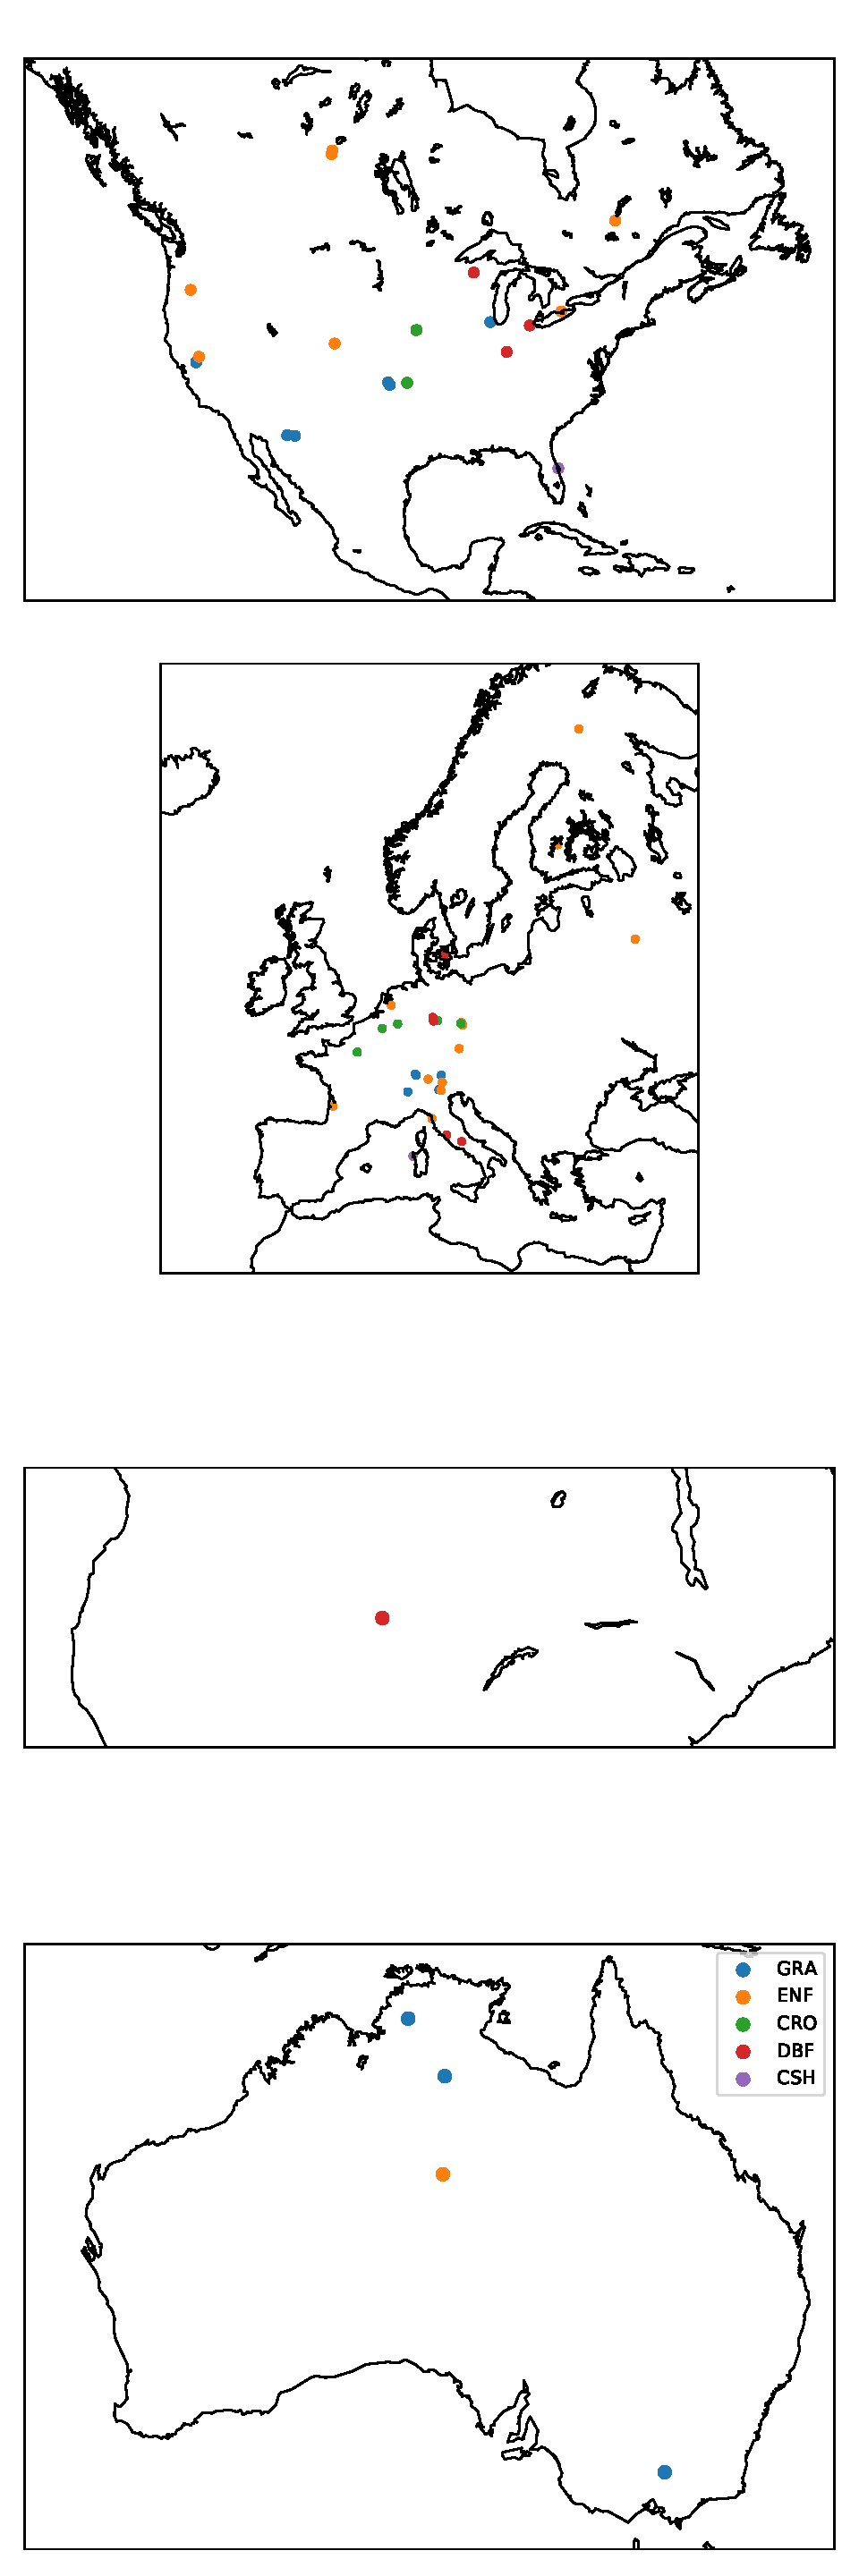
\includegraphics[width=20pc]{./fig01.pdf}
\caption{Plant functional type and location of sites used in analysis. Note should probably just split this into 4 continents (US, Europe, Africa, Australia).}
\label{map_fig}
 \end{figure}p

We restrict our analysis to the daytime (sensible heat > 5 W m$^{-1}$ and shortwave radiation > 50 W m$^{-2}$) when there is no precipitation and the plants are growing (GPP > 10\% of the 95th pecentile). Also, because some sites use half hourly data but some use hourly, we aggregate all data to hourly averages. Only times with good quality control flags are used.

\section{Results}
\label{results}

By construction, the variability in the LAI term (Equation \ref{lai}) contains all model and observational uncertities. LAI also has physical meaning corresponding to ``true'' leaf area, and we expect that it would be approximately $O(1)$. We can have some confidence in our framework, including the assumption of constant uWUE, if calculated LAIs are generally $O(1)$. Figure \ref{lai_fig} presents the histogram of calculated LAIs with outliers (lowest and highest 5\% percent) and unphysical values (LAI $<$ 0.) removed. All remaining LAI values are $O(1)$ which provides confidence in model framework.

\begin{figure}[h]
\centering
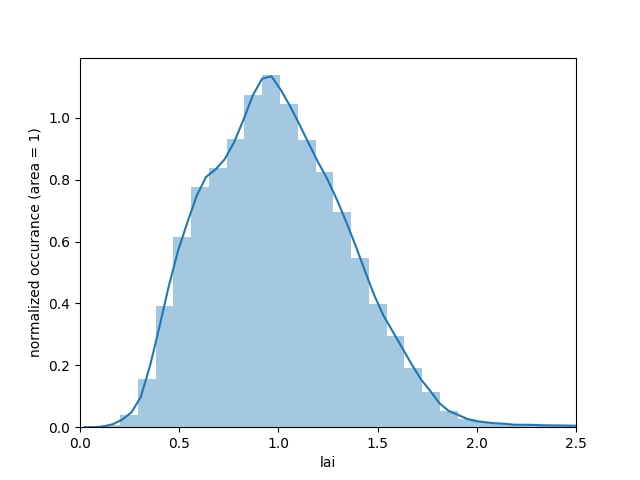
\includegraphics[width=20pc]{./fig02.png}
\caption{Histogram of LAI values calculated for each site and time according to Equation \ref{lai}. The lowest and highest 5\% are removed as outliers, as well as any values below 0. The curve is normalized such that its area is 1.}
\label{lai_fig}
\end{figure}

An additional concern is that the LAI term may in fact be some function of $D$, in which case the dependence would need to be accounted for when taking the derivative. Figure \ref{lai_vpd_fig} plots the joint distrivution of LAI and VPD, and shows that LAI is very weakly a function of VPD. Given this weak dependence, we argue that Equation \ref{d_et} is a valid approxiamtion for ET response to $D$.

% below show histogram of site specific spearmannr? think would be useful 
\begin{figure}[h]
\centering
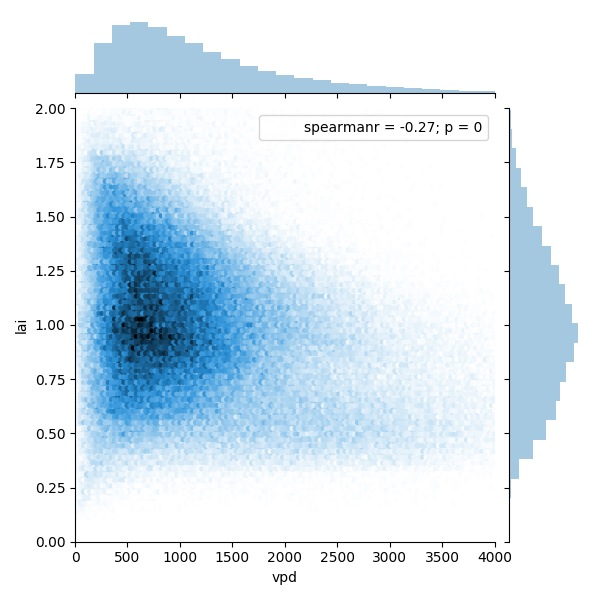
\includegraphics[width=20pc]{./fig03.png}
\caption{The joint distribution of $D$ and LAI. LAI has only a weak dependence on $D$}
\label{lai_vpd_fig}
\end{figure}


Before diving into calculated values of $\frac{\partial \; ET}{\partial \; D}$, it is useful to consider the functional form of Equation \ref{d_et}. There are three terms: a scaling term for the full expression we will call Term 1 ($\frac{g_a \; P}{T(\Delta + \gamma)}$), a relatively constant offset we will call Term 2 ($\frac{c_p}{R_{air}}$), and a variable term we will call Term 3 ($\frac{\gamma c_s }{\text{LAI }1.6 \; R\; \text{ uWUE }} \left( \frac{2 g_1 + \sqrt{D}}{2 (g_1 + \sqrt{D})^2}\right)$). All variables are positive, so the relative magnitude between Term 2 and Term 3 will determine the sign of the derivative, while Term 1 will scale the expression larger or smaller.

In Term 1, $\frac{P}{T} \propto \rho$, so this should vary little relative to $g_a$ and $\Delta$.  $\gamma$ should also be relatively constant, So the scaling term, Term 1, should be primarily a function of $g_a$ and temperature (through the function $\Delta$). While temperature range may vary for PFT, the fucntional form of $\Delta$ will be the same. $g_a$ will vary strongly with PFT due to the importance of surface roughness. However, the coeffiecent of variability for $g_a$ is relatively constant across PFT. So, the influence of $g_a$ on the relative (to the mean) variability of Term 1 is approximately similiar across PFT.

Figure \ref{scale_vary}A shows Term 1 normalized by mean $g_a$ (calcualted for each plant functional type), and confirms that much of the relative variability of Term 1 is contained in the $g_a$ term's relative variability. Additionally, the impact of $T$ on the relative variability increases with increasing $g_a$. % plot every PFT and show they collapse onto the same vurve?

While the relative variability of Term 1 is similiar across PFT, the absolute value of Term 1 varies strongly across PFT. Figure \ref{scale_vary}B shows Term 1 evaluated with the mean $g_a$ for each PFT, and at the range of observed temperatures for each PFT. As expected, for the tree PFTs (DBF, ENF) Term 1 is much larger and the temperature dependence is much stronger. Systematic differences in observed temperatures also cause differences in the average magnitude of Term 1. For example, ENF experiences on average colder temperatures and is thus more likely to have a larger scaling term. Additionally, because std$(g_a) \propto \overline{g_a}$, the spread of Term 1 due to $g_a$ variability will be larger, although this is not shown for simplicity. To summarize, the variability of Term 1 will look like Figure \ref{scale_vary}A for each PFT, but the scale of the x and y-axis will increase or decrease according to Figure \ref{scale_vary}B.
 
\begin{figure}[h]
\centering
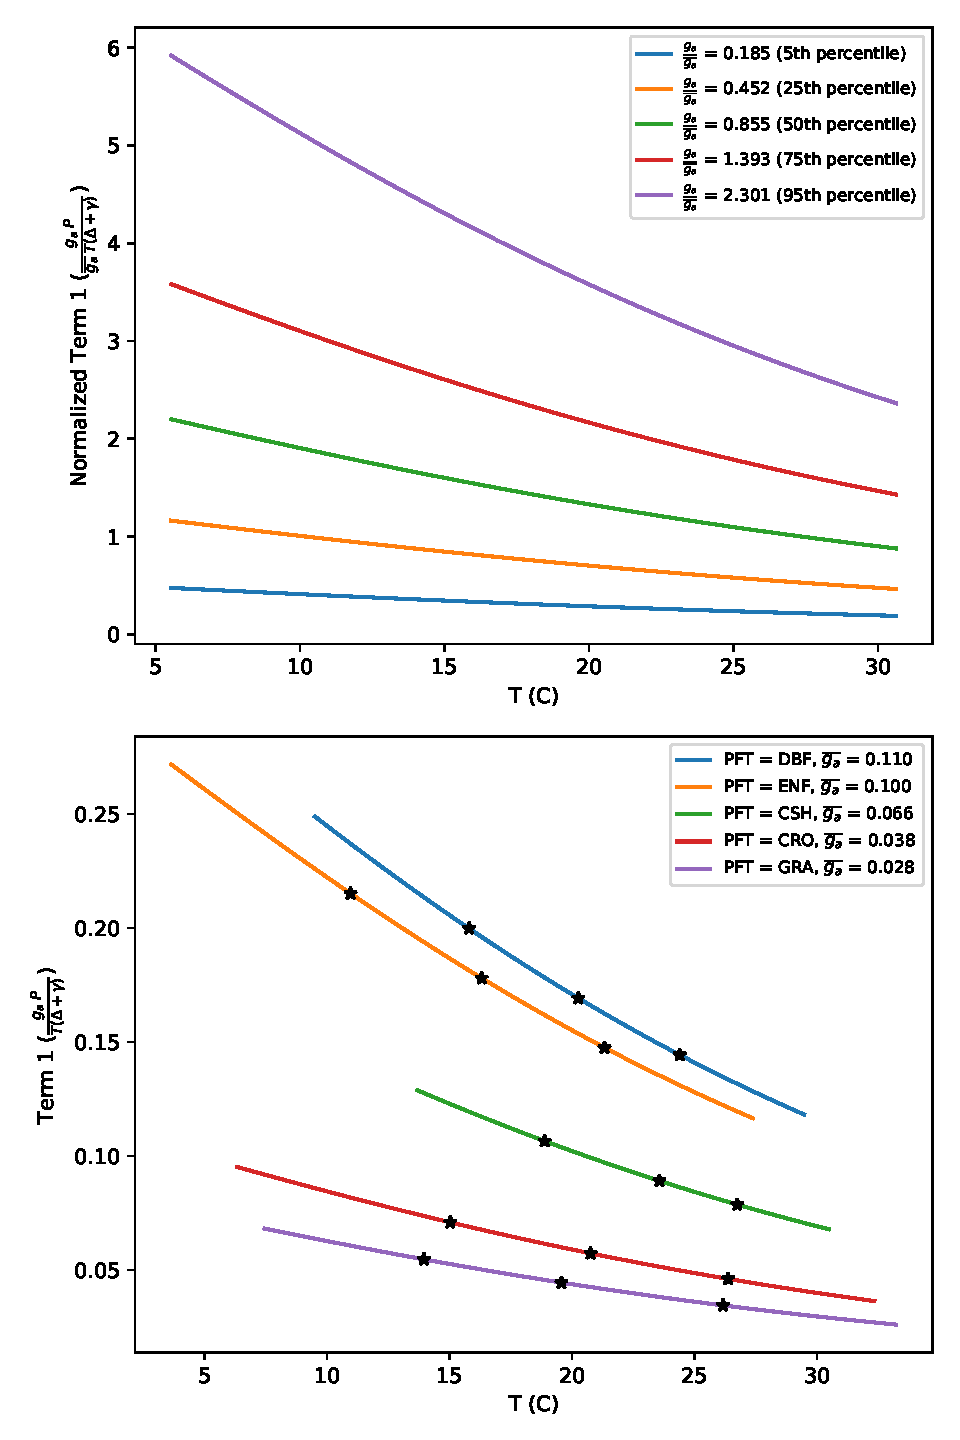
\includegraphics[width=20pc]{./fig04.pdf}
\caption{Primary sources of variability for Term 1. A) Variability within each PFT: Term 1 normalized by mean $g_a$ for each PFT. B) Variability between each PFT: Term 1 evaluated at mean $g_a$ for each PFT. Temperature range is 5-95th percentile for each PFT. Additionally, stars denote the location of the 25th, 50th, and 75th percentiles.}
\label{scale_vary}
\end{figure}

%%%%% replace below with idea:

``just say that vpd effect is approximately linear (except at low VPD), and then say so we are most concerned about when d et/dvpd is zero, as this is the minima. then you can just look at this treshold as a function of LAI, uWUE, and g1.''

Term 2 minus Term 3 determines the sign and magnitude that the scaling Term 1 is multiplied by. If we assume that $c_s$ variability is relatively less than LAI and $D$ variability, then variability within PFT will be soley detmined by LAI and $D$. Figure \ref{term3} shows how (Term 2 - Term 3) varies with $D$ and LAI, as a function of PFT. In Figure \ref{term3}a lower uWUE and LAI shift the disrtribution of (Term 2 - Term 3) towards negative values. Additionally, the smaller $g1$, the greater the relative $D$ dependence of of (Term 2 - Term 3). This is observed most strongly for the ENF PFT, which has the smallest $g1$ (74.31). 


 
\begin{figure}[h]
\centering
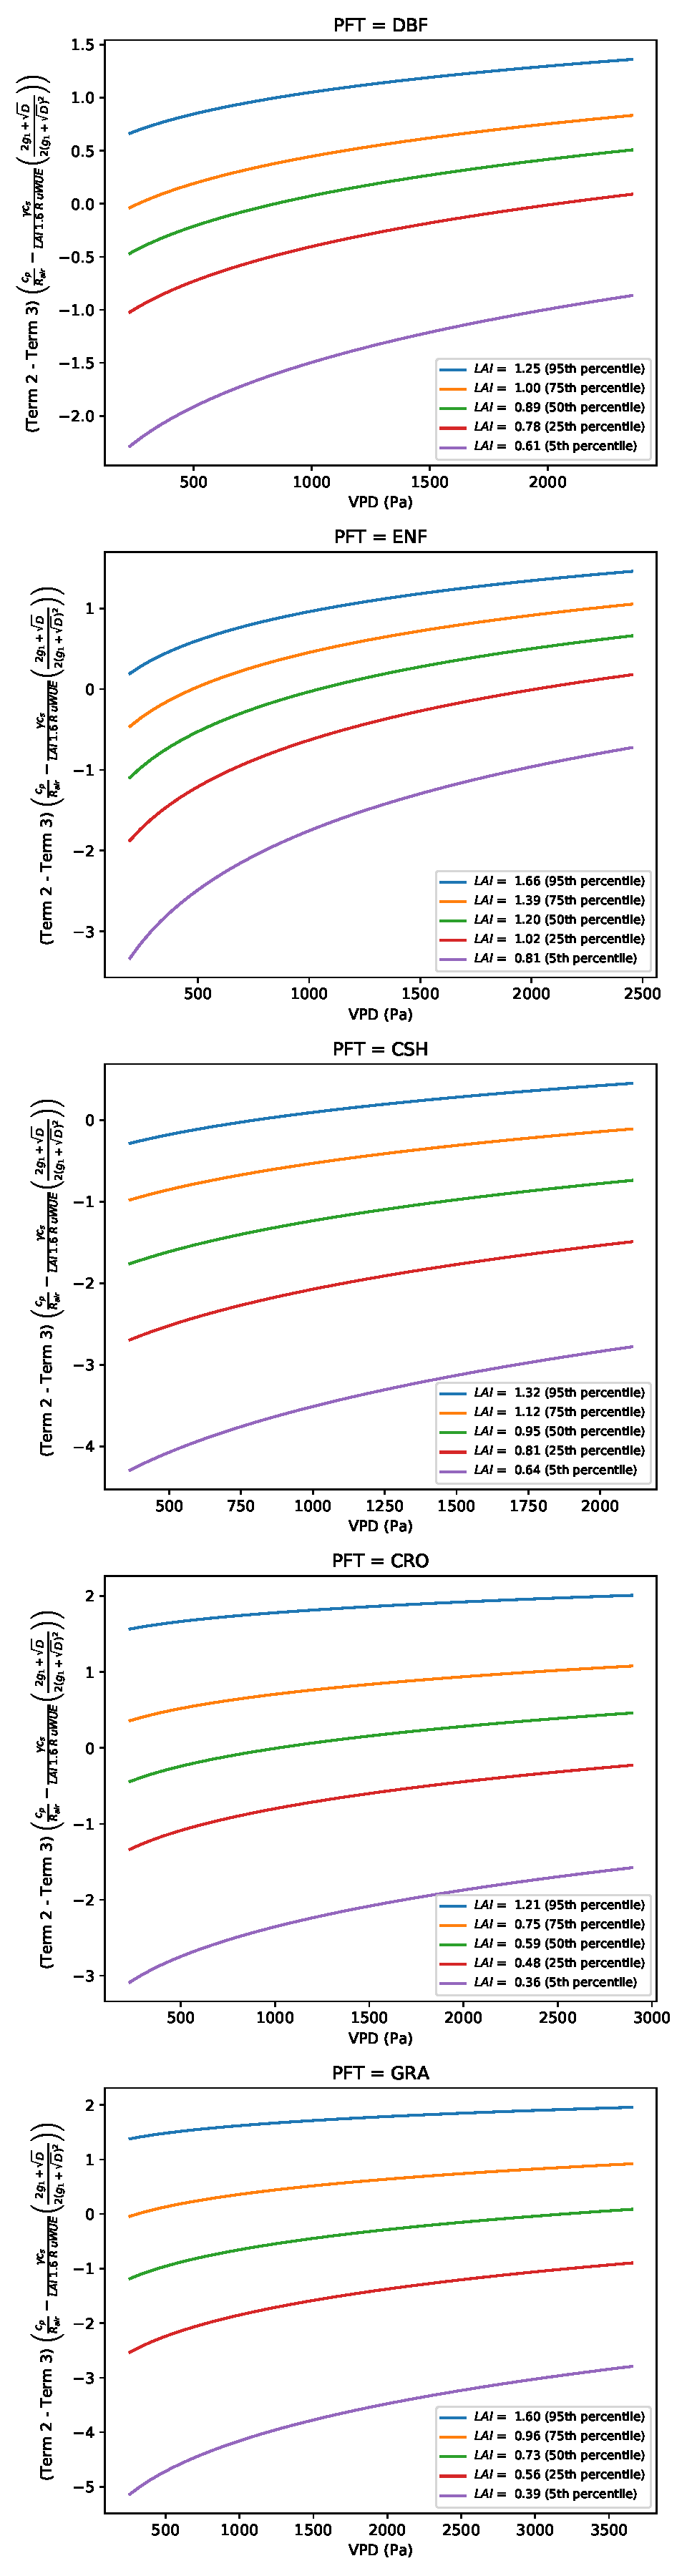
\includegraphics[width=20pc]{./fig05.pdf}
\caption{Sources of variability for Term 2 - Term 3. Top: Term 2 - Term 3 as a function of VPD, with LAI held fixed at PFT averages. The observed range of VPD for each PFT is also shown below the x-axis. Line extent correspondes to 5th and 95th precentiles, while stars denote the location of the 25th, 50th, and 75th percentiles.

Bottom: The location of the minima of ET, as a function of VPD and LAI. Lines and stars denote the distribution of VPD and LAI next to axis, following the same percentiles as above.}
\label{term3}
\end{figure}



Figure \ref{term3}b shows the location of the minima of ET, as a function of LAI and $D$. For any LAI or VPD less (more) than these curves, Term 2 - Term 3 will be negative (positive). It is clear that the portion of VPD observations below these curves will be a strong function of $LAI$. However, we can see some general trends. For CSH, $\frac{\partial \; ET}{\partial \; D}$ should be negative for the vast majority of observed LAI and VPD. The split appears to be more even among ENF, GRA, and DBF, and we might expect a greater frequency of positive $\frac{\partial \; ET}{\partial \; D}$ for CRO. 

Table 3 confirms these expectations for PFT behaviour of $\frac{\partial \; ET}{\partial \; D}$. For all PFTs except for CRO, average $\frac{\partial \; ET}{\partial \; D}$ is less than zero. However, $\frac{\partial \; ET}{\partial \; D}$ evaluated at the average of all variables (e.g. LAI, $T$, $c_s$, $D$) is only negative for CSH and GRA. And, DBF in addition to CRO experiences $\frac{\partial \; ET}{\partial \; D}$ < 0 less than half the time. These observations highlight the effect of the nonlinear function in Figure \ref{term3}: $\frac{\partial \; ET}{\partial \; D}$ has a much steeper slope when the function is negative, and is thus more likely to be large magnitude.
n
The units of $\frac{\partial \; ET}{\partial \; D}$ make it difficult to interpret if $D$ is even a meaningful contributor to ET's variability. To understand $D$'s contribution better, we use a linear approximation and present $\frac{\partial \; ET}{\partial \; D}$ multiplied by $D$'s standard deviation. The range of $D$'s contribution to ET's variability ranges between 16 - 20 W m$^{-2}$ for all PFTs except for CSH, which is about 51 W m$^{-2}$. Another meaningful comparison is to $\frac{\partial \; ET}{\partial \; R} * std(R)$, as net radiation generally the driver of ET (cite joe berry here). For all PFTs except for CSH $D$ contributes between 14.5 - 20.5 \% of $R$'s contribution to variability. For CSH the portion is much larger, about 44 \%. However it is important to note that a linear approximation about a mean base state is probably not a very good approximation across the range of variabilility, so these values are just estimates of $D$'s contribution to ET's variability. 

So far, idealized plots and statistics have illuminated the form of $\frac{\partial \; ET}{\partial \; D}$ and how it varies with PFT. Large mean LAI and uWUE shifts CRO and DBF towards positive $\frac{\partial \; ET}{\partial \; D}$. However, the strongly nonlinear funtion of $\frac{\partial \; ET}{\partial \; D}$ at $\frac{\partial \; ET}{\partial \; D} < 0$ pushes $\overline{\frac{\partial \; ET}{\partial \; D}}$ negative for DBF (it does not do this for CRO because of CRO's high $g1$). ENF's low $g1$ value increases the dependence of $\frac{\partial \; ET}{\partial \; D}$ on $D$, and makes the function more strongly nonlinear. This has the side effect of pushing $\overline{\frac{\partial \; ET}{\partial \; D}}$ negative futher than other PFTs for a given fraction $\frac{\partial \; ET}{\partial \; D} < 0$ and magntiude $\frac{\partial \; ET}{\partial \; D}(\overline{T,\ldots,D})$. GRA shows the opposite behavior; a relatively high $g1$  makes the function more linear, decreasing the magnitude of $\overline{\frac{\partial \; ET}{\partial \; D}}$ for a given fraction $\frac{\partial \; ET}{\partial \; D} < 0$ and magntiude $\frac{\partial \; ET}{\partial \; D}(\overline{T,\ldots,D})$ (although $g_a$ and Term 1 also probably have a role in this). Finally, low $uWUE$ of CSH pushes to toward by far the lowest values $\frac{\partial \; ET}{\partial \; D}$ (Figure \ref{term3}). Variability in $D$ accounts for the largest about of $ET$ variability for CSH. For the other PFTs, $D$ contributes less to $ET$ variaibiliyt, but still represents about 15-20 \% of $R$'s contributions to ET variability.

\begin{table}
\caption{Statistics of $\frac{\partial \; ET}{\partial \; D}$ as a function of PFT.}
\centering
\begin{tabular}{l c c c c c}
  \hline
PFT & $\overline{\frac{\partial \; ET}{\partial \; VPD}}$ & $\frac{\partial \; ET}{\partial \; D}\left(\overline{T, \ldots , D}\right)$ & $\frac{\partial \; ET}{\partial \; D}\left(\overline{T, \ldots , D}\right)*\text{std}(D)$ & $\frac{\frac{\partial \; ET}{\partial \; D}\left(\overline{T, \ldots , D}\right)*\text{std}(D)}{ \frac{\partial \; ET}{\partial \; R}\left(\overline{T, \ldots , D}\right)*\text{std}(R)}$ & fraction $\frac{\partial \; ET}{\partial \; VPD} < 0.$ \\
  \hline
CRO & 0.000853 & 0.026241 & 18.523659 & 0.203022 & 0.473311\\
CSH & -0.108234 & -0.091526 & 50.861613 & 0.439379 & 0.931660\\
DBF & -0.012727 & 0.013794 & 19.734435 & 0.164241 & 0.461674\\
ENF & -0.034087 & 0.000706 & 16.611852 & 0.148548 & 0.534425\\
GRA & -0.019637 & -0.000921 & 16.798083 & 0.173552 & 0.631735\\
\hline
\multicolumn{2}{l}{$^{a}$Footnote text here.}  

  
\end{tabular}
\end{table}


\subsection{Full observations of $\frac{\partial \; ET}{\partial \; D}$}

Now that we have an intuitive understanding of $\frac{\partial \; ET}{\partial \; D}$'s behavior, we are equipped to intepret fully realistic plots of $\frac{\partial \; ET}{\partial \; D}$ for each PFT. Figure \ref{real} presents calculated $\frac{\partial \; ET}{\partial \; D}$ where, unless otherwise noted, all variables in Equation \ref{d_et} are allowed to vary. Each column is a different quantity related to $\frac{\partial \; ET}{\partial \; D}$, and each row is a different PFT.

The full observations generally confirm expectations from Section \ref{results}. CRO has the most postitive values of $\frac{\partial \; ET}{\partial \; D}$, $\frac{\partial \; ET}{\partial \; D}$ is almost always negative for CSH, and reponse depends more with the environmental conditions for the other PFTs (especially ENF). Through the columns of Figure \ref{real} we can see the impact of LAI and $g_a$ on the variability of $\frac{\partial \; ET}{\partial \; D}$. $g_a$'s (columns 1 and 3) scaling alters the magnitude considerably. $LAI$ (columns 2 and 3) variability adds a lot of additional noise to the signal of $\frac{\partial \; ET}{\partial \; D}$, which is slightly undesirable given LAI's role in representing model and observational uncertainty. However, the general story with the noise appears to match the cleaner signal when $LAI$ is help constant and $D_{ETmin}$ is clearly visible \explain{I really need to make these pltos better - way too much overlapping of points that hurts the story}. One exception is possibly with GRA, for which uncertainty is high and causes the full complexity plots (Columns 1 and 2) to not match well with LAI held fixed (Columns 3 and 4).

For ENF and GRA $D_{ETmin}$ does not appear to be only a function of LAI. It turns out that the site to site variaibility in $\gamma$ causes $D_{ETmin}$ to vary, which is not discussed in the pregious section. The impact is observable in both ENF and GRA, but especially for ENF which has a larger $\frac{\partial^2 \; ET}{\partial^2 \; D}$ than the other PFTs. 

In general the full complexity plots of $\frac{\partial \; ET}{\partial \; D}$ match our expectations, even with the large sensitivty to LAI measures of uncertainty observed in Figure \ref{term3}. Our LAI-based method of uncertainty propogation blurrs the idealized expectations the most for GRA, and also has a considerable effect for CRO. We therefor have the most confidence in our conclusion based on Equation \ref{d_et} for PFTS CSH, DBF, and ENF, as the full complexity plots with uncertainty included closely match the story when LAI is held fixed. **see somewhat preferred alternate figure \ref{real2} \explain{I think I like this more as thinking in terms of T and RH is easier. However, I used the other plot because Fig 5 does not discuss things in terms of temperature, as this would make things more complicated (adding another diminsion). I could just include both versions of figure 6 though (using figure 6a as a bridge to figure 6b)}.
\begin{figure}[h]
\centering
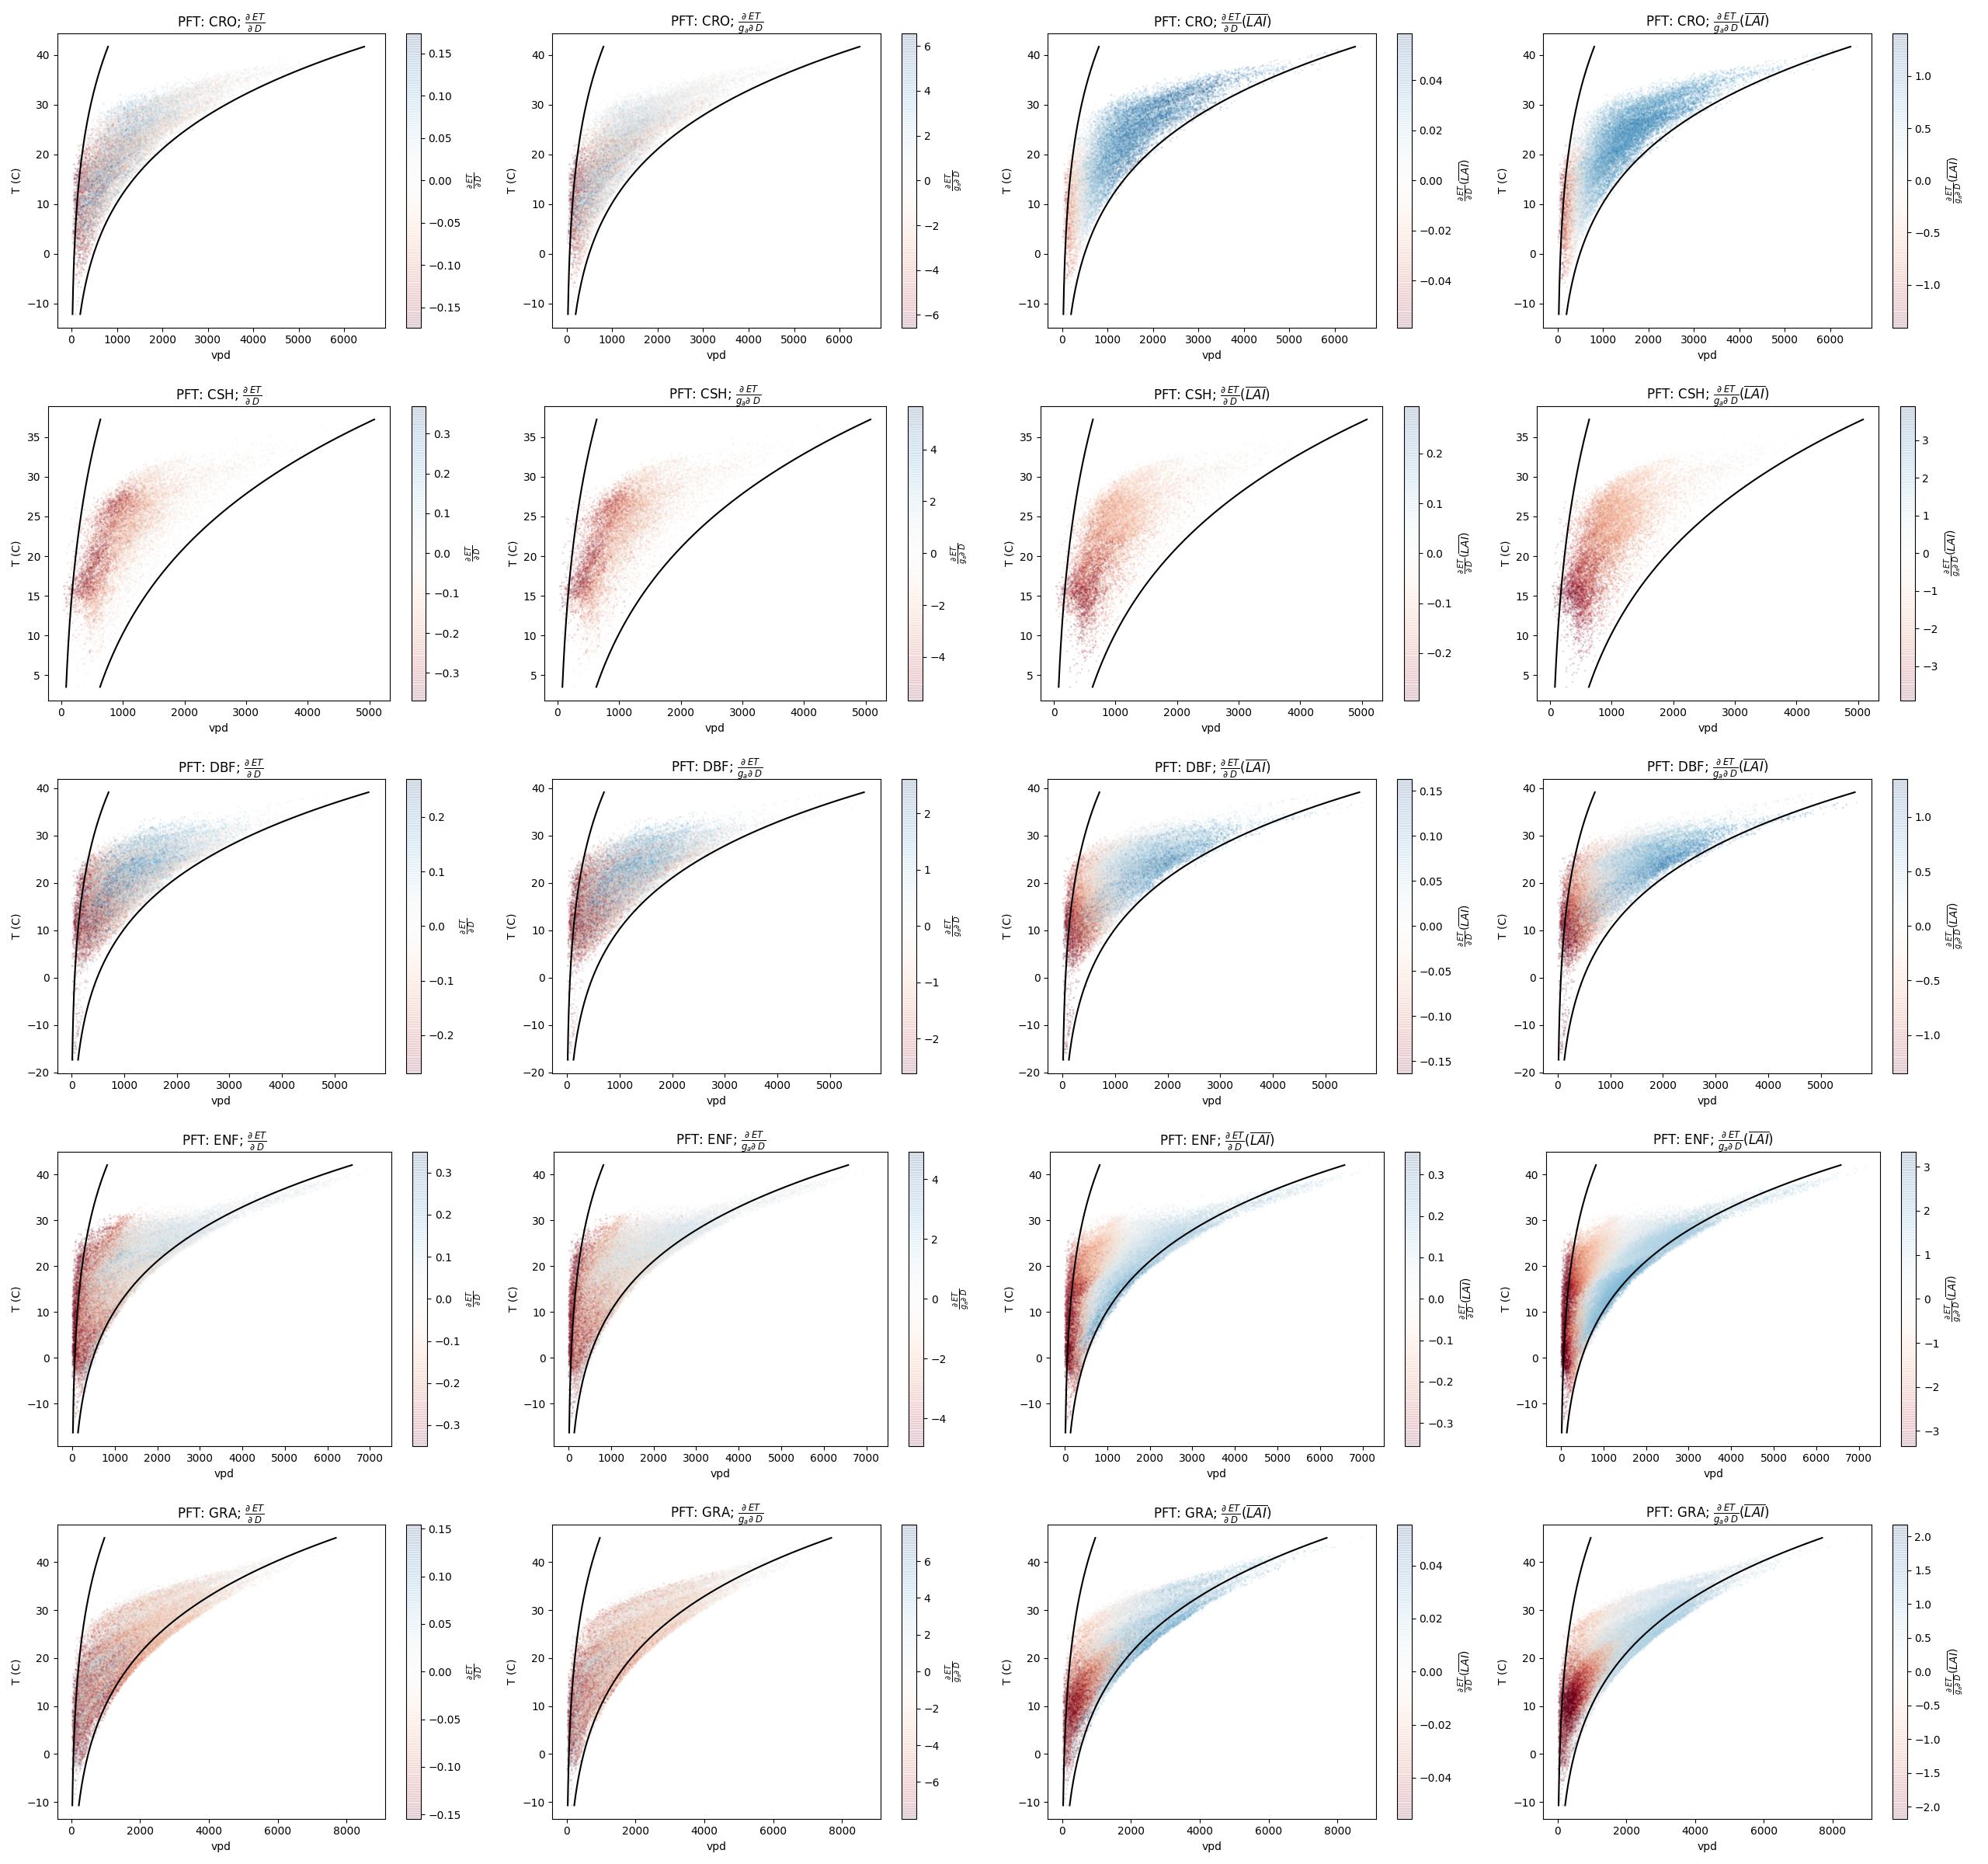
\includegraphics[width=\textwidth]{./fig06.png}
\caption{Scatter plots of $\frac{\partial \; ET}{\partial \; D}$. Each row is a different PFT, and each column is a different quantity related to $\frac{\partial \; ET}{\partial \; D}$, as labelled: Column 1 - $\frac{\partial \; ET}{\partial \; D}$; Column 2 - $\frac{\partial \; ET}{\partial \; D}$ normalized by $g_a$; Column 3 - $\frac{\partial \; ET}{\partial \; D}$ with LAI held fixed at PFT average; and Column 4 - $\frac{\partial \; ET}{\partial \; D}$ normalized by $g_a$ and with LAI held fixed. For reference, lines corresponding to RH = 20\% and RH = 90 \% are drawn. Please note differences in the colorbar scale.}
\label{real}
\end{figure}

\begin{figure}[h]
\centering
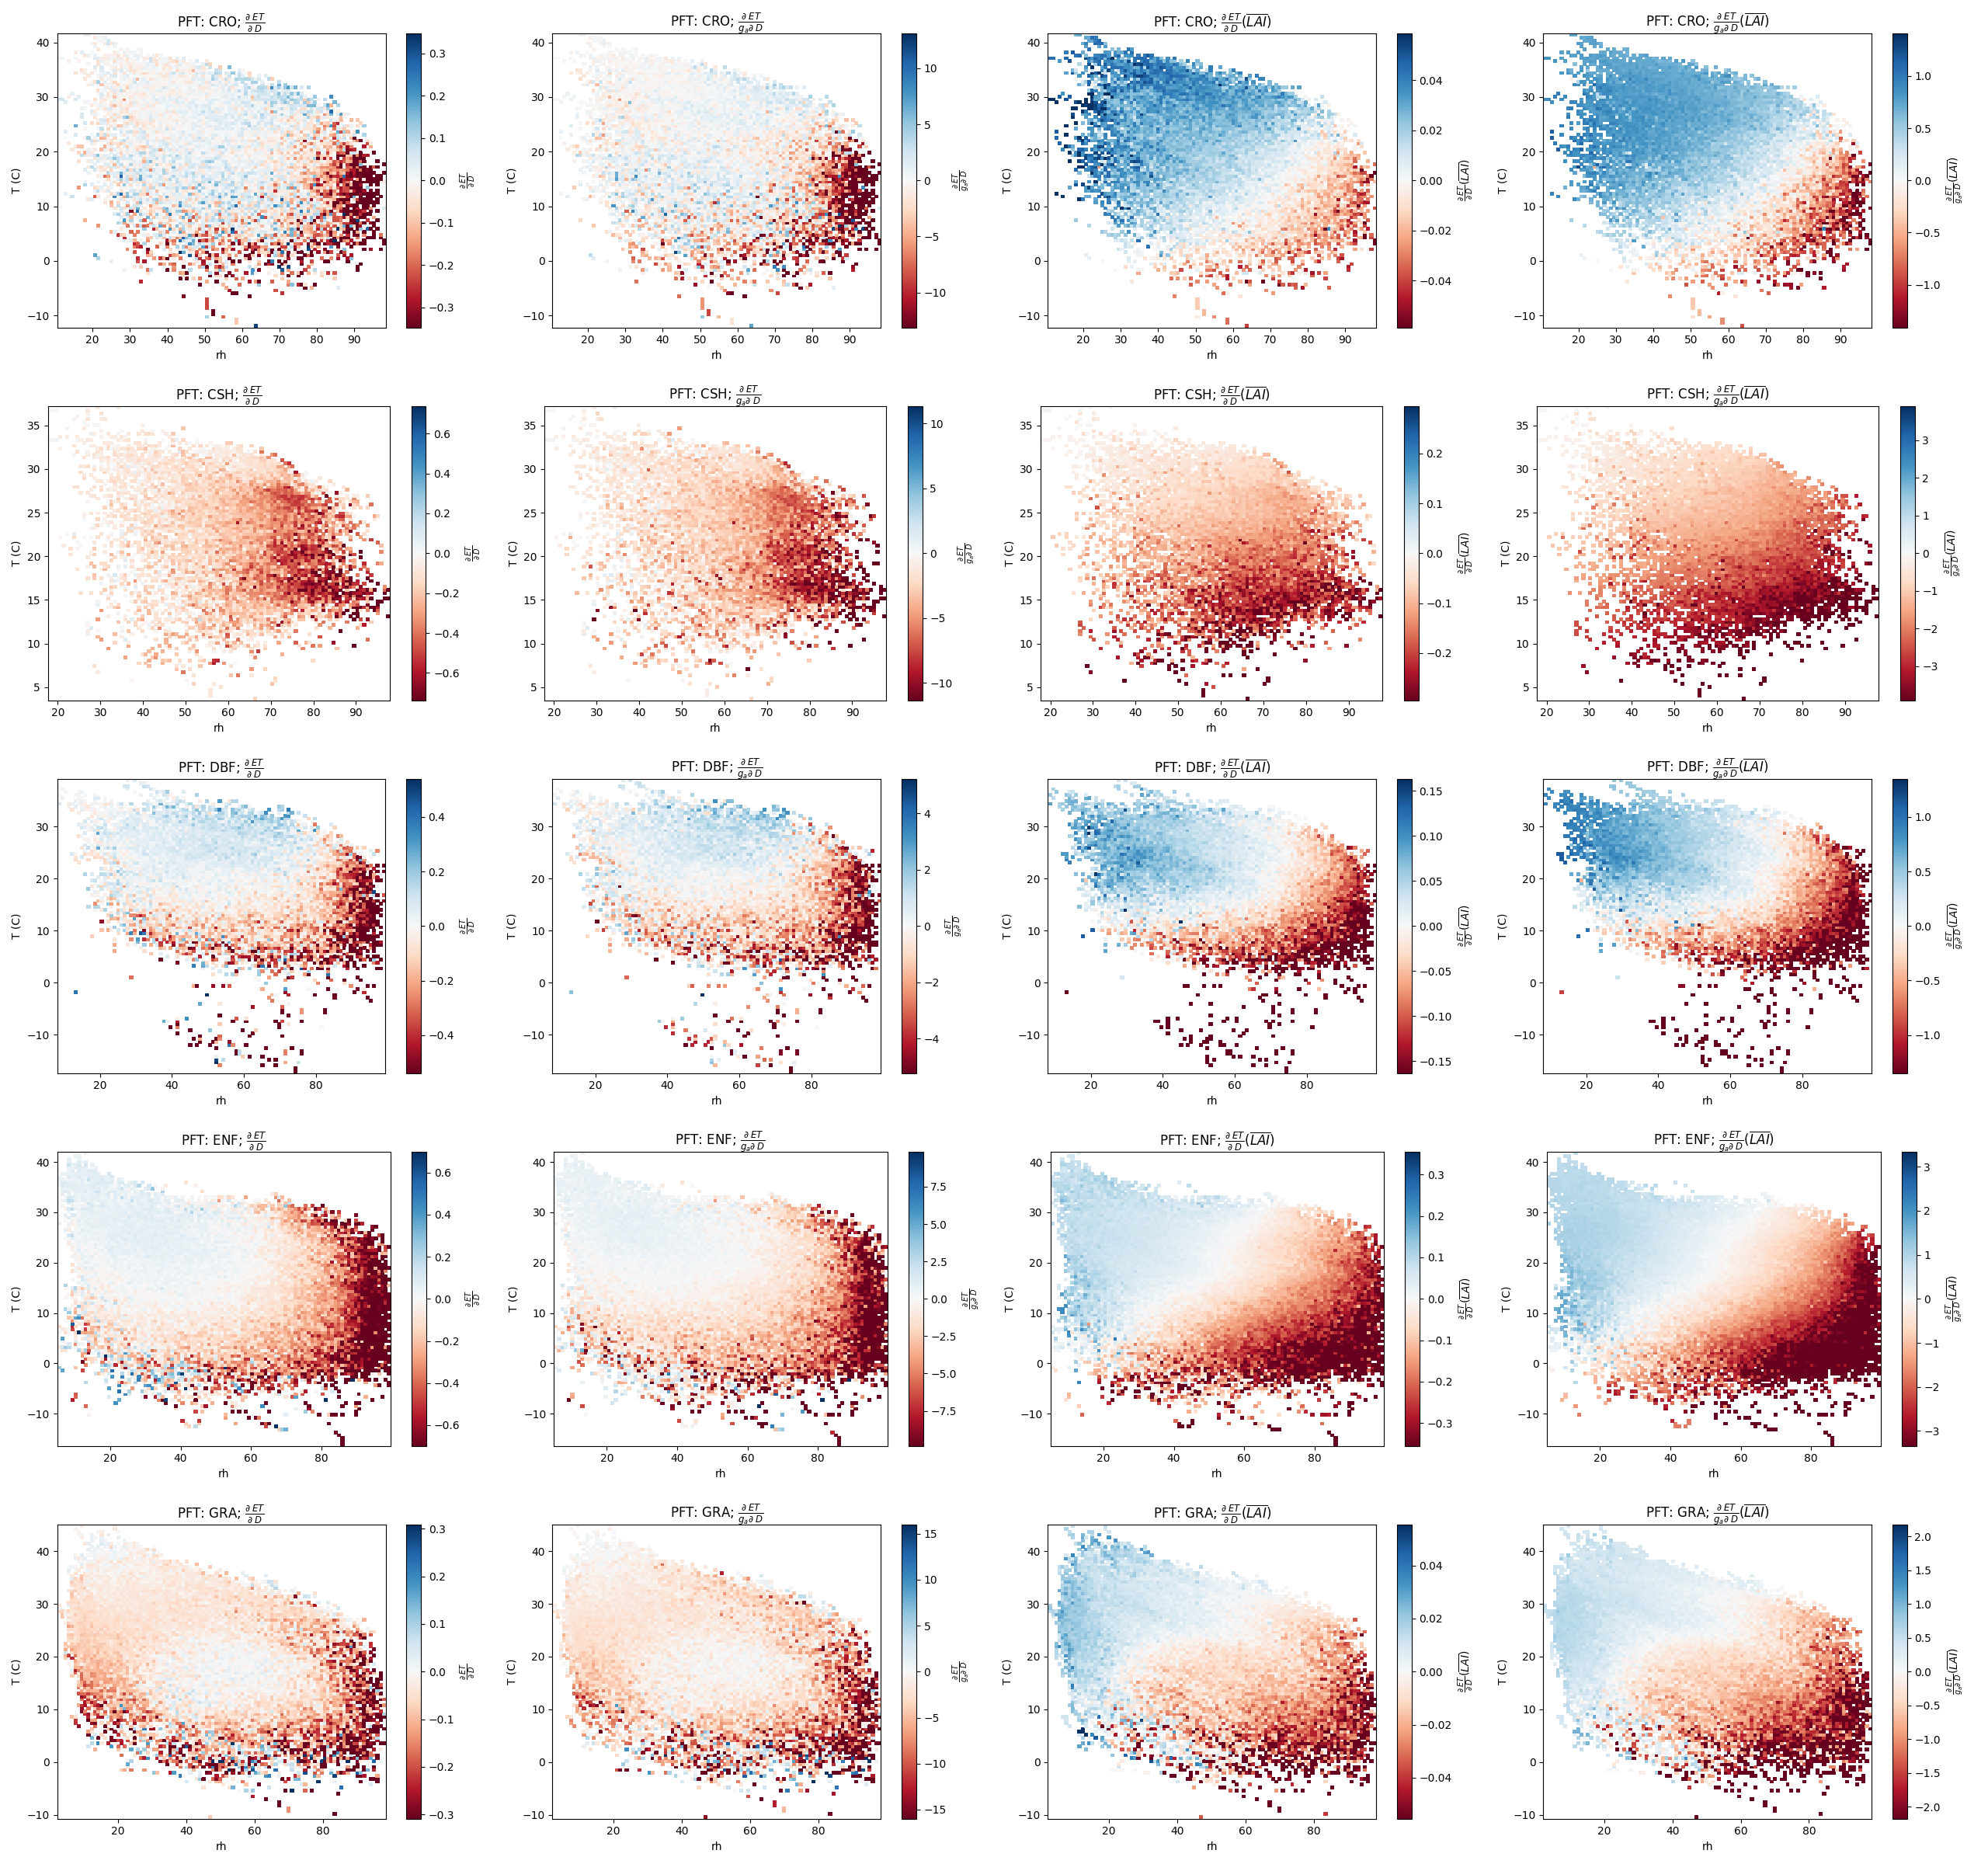
\includegraphics[width=\textwidth]{./fig06b.png}
\caption{****alternate Fig 06****  Scatter plots of $\frac{\partial \; ET}{\partial \; D}$. Each row is a different PFT, and each column is a different quantity related to $\frac{\partial \; ET}{\partial \; D}$, as labelled. If I end up using this, I could also draw on the curve of $D_{ETmin}$ with $\overline{LAI}$. }
\label{real2}
\end{figure}


\section{Conclusions} \explain{also need to flesh this section out}

The idealized representation of ET used here is successful in developing intuition for how ET responds to changes in $D$. This intuition will aid the community in interpreting observations and output from sophisticated full complexity climate models.

The idealized framework leads to the following general conclusions:
\begin{itemize}
  \item Aerodynamic resistance plays an important role of scaling $\frac{\partial \; ET}{\partial \; D}$. This is a leading order effect for observing higher magnitude reponses in DBF and ENF.
\item In general, CSH has the most negative (i.e. ET reduced) response to increases in $D$ (atmospheric drying). So CSH plants will almost always try and conserve water, effectivey reducing ET with dry atmospheric perturbation.
\item CRO has the most postive response (i.e. ET increased) in response to increases in $D$. This is consistent with CROs that may be evolved or bred to thrive in non-water-limited environments.
\item The reponse is more a function of the environment for DBF, ENF, and GRA. Because as VPD increases the response is more likely to be postive, if RH is fixed then the reponse will be more likely to be positive at warmer T, or if T is fixed the response is more likely to be positive with decreasing RH.
\item ENF has the strongest dependence on environmental conditions due to its small $g1$.
\item Model and observational uncertainty is highest for GRA and CRO, so conlusions about those PFTs should be tempered.
\item However, inclusion of uncertainty doesn't alter conclusions about DBF, ENF, and CSH.
\end{itemize}

The intuition developed using this framework can be used to understand how the land surface will respond and contribute to changes in the environment. 

  

%%
%% Enter Figures and Tables near as possible to where they are first mentioned:
%
% DO NOT USE \psfrag or \subfigure commands.
%
% Figure captions go below the figure.
% Table titles go above tables;  other caption information
%  should be placed in last line of the table, using
% \multicolumn2l{$^a$ This is a table note.}
%
%----------------
% EXAMPLE FIGURE
%
% \begin{figure}[h]
% \centering
% when using pdflatex, use pdf file:
% \includegraphics[width=20pc]{figsamp.pdf}
%
% when using dvips, use .eps file:
% \includegraphics[width=20pc]{figsamp.eps}
%
% \caption{Short caption}
% \label{figone}
%  \end{figure}
%
% ---------------
% EXAMPLE TABLE
%
% \begin{table}
% \caption{Time of the Transition Between Phase 1 and Phase 2$^{a}$}
% \centering
% \begin{tabular}{l c}
% \hline
%  Run  & Time (min)  \\
% \hline
%   $l1$  & 260   \\
%   $l2$  & 300   \\
%   $l3$  & 340   \\
%   $h1$  & 270   \\
%   $h2$  & 250   \\
%   $h3$  & 380   \\
%   $r1$  & 370   \\
%   $r2$  & 390   \\
% \hline
% \multicolumn{2}{l}{$^{a}$Footnote text here.}
% \end{tabular}
% \end{table}

%% SIDEWAYS FIGURE and TABLE 
% AGU prefers the use of {sidewaystable} over {landscapetable} as it causes fewer problems.
%
% \begin{sidewaysfigure}
% \includegraphics[width=20pc]{figsamp}
% \caption{caption here}
% \label{newfig}
% \end{sidewaysfigure}
% 
%  \begin{sidewaystable}
%  \caption{Caption here}
% \label{tab:signif_gap_clos}
%  \begin{tabular}{ccc}
% one&two&three\\
% four&five&six
%  \end{tabular}
%  \end{sidewaystable}

%% If using numbered lines, please surround equations with \begin{linenomath*}...\end{linenomath*}
%\begin{linenomath*}
%\begin{equation}
%y|{f} \sim g(m, \sigma),
%\end{equation}
%\end{linenomath*}

%%% End of body of article

%%%%%%%%%%%%%%%%%%%%%%%%%%%%%%%%
%% Optional Appendix goes here
%
% The \appendix command resets counters and redefines section heads
%
% After typing \appendix
%
%\section{Here Is Appendix Title}
% will show
% A: Here Is Appendix Title
%
%\appendix
%\section{Here is a sample appendix}

%%%%%%%%%%%%%%%%%%%%%%%%%%%%%%%%%%%%%%%%%%%%%%%%%%%%%%%%%%%%%%%%
%
% Optional Glossary, Notation or Acronym section goes here:
%
%%%%%%%%%%%%%%  
% Glossary is only allowed in Reviews of Geophysics
%  \begin{glossary}
%  \term{Term}
%   Term Definition here
%  \term{Term}
%   Term Definition here
%  \term{Term}
%   Term Definition here
%  \end{glossary}

%
%%%%%%%%%%%%%%
% Acronyms
%   \begin{acronyms}
%   \acro{Acronym}
%   Definition here
%   \acro{EMOS}
%   Ensemble model output statistics 
%   \acro{ECMWF}
%   Centre for Medium-Range Weather Forecasts
%   \end{acronyms}

%
%%%%%%%%%%%%%%
% Notation 
%   \begin{notation}
%   \notation{$a+b$} Notation Definition here
%   \notation{$e=mc^2$} 
%   Equation in German-born physicist Albert Einstein's theory of special
%  relativity that showed that the increased relativistic mass ($m$) of a
%  body comes from the energy of motion of the body—that is, its kinetic
%  energy ($E$)—divided by the speed of light squared ($c^2$).
%   \end{notation}




%%%%%%%%%%%%%%%%%%%%%%%%%%%%%%%%%%%%%%%%%%%%%%%%%%%%%%%%%%%%%%%%
%
%  ACKNOWLEDGMENTS
%
% The acknowledgments must list:
%
% •	All funding sources related to this work from all authors
%
% •	Any real or perceived financial conflicts of interests for any
%	author
%
% •	Other affiliations for any author that may be perceived as
% 	having a conflict of interest with respect to the results of this
% 	paper.
%
% •	A statement that indicates to the reader where the data
% 	supporting the conclusions can be obtained (for example, in the
% 	references, tables, supporting information, and other databases).
%
% It is also the appropriate place to thank colleagues and other contributors. 
% AGU does not normally allow dedications.


\acknowledgments
This work used eddy covariance data acquired and shared by the FLUXNET community, including these networks: AmeriFlux, AfriFlux, AsiaFlux, CarboAfrica, CarboEuropeIP, CarboItaly, CarboMont, ChinaFlux, Fluxnet-Canada, GreenGrass, ICOS, KoFlux, LBA, NECC, OzFlux-TERN, TCOS-Siberia, and USCCC. The ERA-Interim reanalysis data are provided by ECMWF and processed by LSCE. The FLUXNET eddy covariance data processing and harmonization was carried out by the European Fluxes Database Cluster, AmeriFlux Management Project, and Fluxdata project of FLUXNET, with the support of CDIAC and ICOS Ecosystem Thematic Center, and the OzFlux, ChinaFlux and AsiaFlux offices.


%% ------------------------------------------------------------------------ %%
%% Citations

% Please use ONLY \citet and \citep for reference citations.
% DO NOT use other cite commands (e.g., \cite, \citeyear, \nocite, \citealp, etc.).


%% Example \citet and \citep:
%  ...as shown by \citet{Boug10}, \citet{Buiz07}, \citet{Fra10},
%  \citet{Ghel00}, and \citet{Leit74}. 

%  ...as shown by \citep{Boug10}, \citep{Buiz07}, \citep{Fra10},
%  \citep{Ghel00, Leit74}. 

%  ...has been shown \citep [e.g.,][]{Boug10,Buiz07,Fra10}.



%%  REFERENCE LIST AND TEXT CITATIONS
%
% Either type in your references using
%
% \begin{thebibliography}{}
% \bibitem[{\textit{Kobayashi et~al.}}(2003)]{R2013} Kobayashi, T.,
% Tran, A.~H., Nishijo, H., Ono, T., and Matsumoto, G.  (2003).
% Contribution of hippocampal place cell activity to learning and
% formation of goal-directed navigation in rats. \textit{Neuroscience}
% 117, 1025--1035.
%
% \bibitem{}
% Text
% \end{thebibliography}
%
%%%%%%%%%%%%%%%%%%%%%%%%%%%%%%%%%%%%%%%%%%%%%%%
% Or, to use BibTeX:
%
% Follow these steps
%
% 1. Type in \bibliography{<name of your .bib file>} 
%    Run LaTeX on your LaTeX file.
%
% 2. Run BiBTeX on your LaTeX file.
%
% 3. Open the new .bbl file containing the reference list and
%   copy all the contents into your LaTeX file here.
%
% 4. Run LaTeX on your new file which will produce the citations.
%
% AGU does not want a .bib or a .bbl file. Please copy in the contents of your .bbl file here.


%% After you run BibTeX, Copy in the contents of the .bbl file here:


%%%%%%%%%%%%%%%%%%%%%%%%%%%%%%%%%%%%%%%%%%%%%%%%%%%%%%%%%%%%%%%%%%%%%
% Track Changes:
% To add words, \added{<word added>}
% To delete words, \deleted{<word deleted>}
% To replace words, \replace{<word to be replaced>}{<replacement word>}
% To explain why change was made: \explain{<explanation>} This will put
% a comment into the right margin.

%%%%%%%%%%%%%%%%%%%%%%%%%%%%%%%%%%%%%%%%%%%%%%%%%%%%%%%%%%%%%%%%%%%%%
% At the end of the document, use \listofchanges, which will list the
% changes and the page and line number where the change was made.

% When final version, \listofchanges will not produce anything,
% \added{<word or words>} word will be printed, \deleted{<word or words} will take away the word,
% \replaced{<delete this word>}{<replace with this word>} will print only the replacement word.
%  In the final version, \explain will not print anything.
%%%%%%%%%%%%%%%%%%%%%%%%%%%%%%%%%%%%%%%%%%%%%%%%%%%%%%%%%%%%%%%%%%%%%

%%%
\listofchanges
%%%

\end{document}

%%%%%%%%%%%%%%%%%%%%%%%%%%%%%%%%%%%%%
%% Supporting Information
%% (Optional) See AGUSuppInfoSamp.tex/pdf for requirements 
%% for Supporting Information.
%%%%%%%%%%%%%%%%%%%%%%%%%%%%%%%%%%%%%



%%%%%%%%%%%%%%%%%%%%%%%%%%%%%%%%%%%%%%%%%%%%%%%%%%%%%%%%%%%%%%%

More Information and Advice:

%% ------------------------------------------------------------------------ %%
%
%  SECTION HEADS
%
%% ------------------------------------------------------------------------ %%

% Capitalize the first letter of each word (except for
% prepositions, conjunctions, and articles that are
% three or fewer letters).

% AGU follows standard outline style; therefore, there cannot be a section 1 without
% a section 2, or a section 2.3.1 without a section 2.3.2.
% Please make sure your section numbers are balanced.
% ---------------
% Level 1 head
%
% Use the \section{} command to identify level 1 heads;
% type the appropriate head wording between the curly
% brackets, as shown below.
%
%An example:
%\section{Level 1 Head: Introduction}
%
% ---------------
% Level 2 head
%
% Use the \subsection{} command to identify level 2 heads.
%An example:
%\subsection{Level 2 Head}
%
% ---------------
% Level 3 head
%
% Use the \subsubsection{} command to identify level 3 heads
%An example:
%\subsubsection{Level 3 Head}
%
%---------------
% Level 4 head
%
% Use the \subsubsubsection{} command to identify level 3 heads
% An example:
%\subsubsubsection{Level 4 Head} An example.
%
%% ------------------------------------------------------------------------ %%
%
%  IN-TEXT LISTS
%
%% ------------------------------------------------------------------------ %%
%
% Do not use bulleted lists; enumerated lists are okay.
% \begin{enumerate}
% \item
% \item
% \item
% \end{enumerate}
%
%% ------------------------------------------------------------------------ %%
%
%  EQUATIONS
%
%% ------------------------------------------------------------------------ %%

% Single-line equations are centered.
% Equation arrays will appear left-aligned.

Math coded inside display math mode \[ ...\]
 will not be numbered, e.g.,:
 \[ x^2=y^2 + z^2\]

 Math coded inside \begin{equation} and \end{equation} will
 be automatically numbered, e.g.,:
 \begin{equation}
 x^2=y^2 + z^2
 \end{equation}


% To create multiline equations, use the
% \begin{eqnarray} and \end{eqnarray} environment
% as demonstrated below.
\begin{eqnarray}
  x_{1} & = & (x - x_{0}) \cos \Theta \nonumber \\
        && + (y - y_{0}) \sin \Theta  \nonumber \\
  y_{1} & = & -(x - x_{0}) \sin \Theta \nonumber \\
        && + (y - y_{0}) \cos \Theta.
\end{eqnarray}

%If you don't want an equation number, use the star form:
%\begin{eqnarray*}...\end{eqnarray*}

% Break each line at a sign of operation
% (+, -, etc.) if possible, with the sign of operation
% on the new line.

% Indent second and subsequent lines to align with
% the first character following the equal sign on the
% first line.

% Use an \hspace{} command to insert horizontal space
% into your equation if necessary. Place an appropriate
% unit of measure between the curly braces, e.g.
% \hspace{1in}; you may have to experiment to achieve
% the correct amount of space.


%% ------------------------------------------------------------------------ %%
%
%  EQUATION NUMBERING: COUNTER
%
%% ------------------------------------------------------------------------ %%

% You may change equation numbering by resetting
% the equation counter or by explicitly numbering
% an equation.

% To explicitly number an equation, type \eqnum{}
% (with the desired number between the brackets)
% after the \begin{equation} or \begin{eqnarray}
% command.  The \eqnum{} command will affect only
% the equation it appears with; LaTeX will number
% any equations appearing later in the manuscript
% according to the equation counter.
%

% If you have a multiline equation that needs only
% one equation number, use a \nonumber command in
% front of the double backslashes (\\) as shown in
% the multiline equation above.

% If you are using line numbers, remember to surround
% equations with \begin{linenomath*}...\end{linenomath*}

%  To add line numbers to lines in equations:
%  \begin{linenomath*}
%  \begin{equation}
%  \end{equation}
%  \end{linenomath*}



